%!TEX root = ../template.tex
%%%%%%%%%%%%%%%%%%%%%%%%%%%%%%%%%%%%%%%%%%%%%%%%%%%%%%%%%%%%%%%%%%%%
%% chapter4.tex
%% NOVA thesis document file
%%
%% Chapter with lots of dummy text
%%%%%%%%%%%%%%%%%%%%%%%%%%%%%%%%%%%%%%%%%%%%%%%%%%%%%%%%%%%%%%%%%%%%

\typeout{NT FILE chapter4.tex}%

\chapter{Workplan}\label{cha:workplan}

To provide a clear overwiew of thr workplan, we create a Gantt chart, displayed in Figure \ref{fig:gantt}, and a table with the tasks and their respective description and tasks dependency. Our workplan is desing for an estimated effort similar to the compleplated work for a Master Thesis, corresponding to 30 ECTS, meaning that we plan to spend 840 hours of work (30 ECTS * 28 hours/ECTS), for which we account for the possibility of a margin of error of 10\% in the total time. 

\section{Protopype Development}
To mitigate the risk of not being able to complete the work in the estimated time, we divided our solution into phases:
\begin{itemize}
    \item \textbf{Phase 1:} Firsly, we will implement the prototype of the \textit{Unobservability Scheduler} with basic functionalities and a randomized response-based mechanisms. In this phase, we prosume to spend a reasonable amount of time setting up and understading Tor's or MIRACE's codebase, depending on the approach we take. With this basic differntial private scheduler, we will already be able to test the basic functionalities of the system, and we will be able to evaluate the performance of the system in terms of privacy and utility. We also want to provide detailed evidence of the impact of each parameter. This way, this prototype will work as reference of the system's performance and will be used to compare with the final version of the system. Therefore, we will have to develop our benchmarking tools and extract data from this prototype.
    \item \textbf{Phase 2:} In this phase, we will extend Phase 1 Protopype and add all necessary parameters. We will start by implementing the static paramenters, as we consider to be easier to implement and less probable to generate unexpected results, due to its static nature. After that, we will implement the dynamic parameters, which will require more time to implement and test. We will also implement the benchmarking tools and extract data from this prototype. Finally, we will compare the results of the two prototypes and evaluate the impact of each parameter in the system's performance and what values do we consider to be the best for each parameter.
\end{itemize}

Upon completing these development phases, particular elements of the solution will be subject to thorough analysis and meticulous implementation:
\begin{itemize}
    \item \textbf{Differential Privacy: } The main focus of this work is to provide a solution that is able to provide formal privacy guarantees to anonymization network's users. Formal privacy guarantees are a important aspect of our system, as it will provide a clear understanding of the privacy guarantees that users have when using our system. Therefore, we will have to implement the differential privacy mechanisms and evaluate its impact in the system's performance.
    \item \textbf{Flexible Configuration \& Parameterization: } Another important aspect of the work we want to develop is the ability to provide flexible behaviour to the system. This flexibility can be divided into two main subjects: the users, and the correspondent needs and preferences, are one source of flexibility and we consider important to provide a system that can be easily configured by the user and fit his needs. On the other hand, the system itself should be able to adapt to the real-time conditions that it is subject to. For example, the system should be able to adapt to the network's jitter and latency, and adapt the noise added to the messages accordingly, by modifying the privacy parameters. Therefore, our system will have a flexible configuration and parameterization, and a vast number of parameters lead to a vast range of tests that we will have to perform.  
\end{itemize}


\begin{figure}
    \centering
    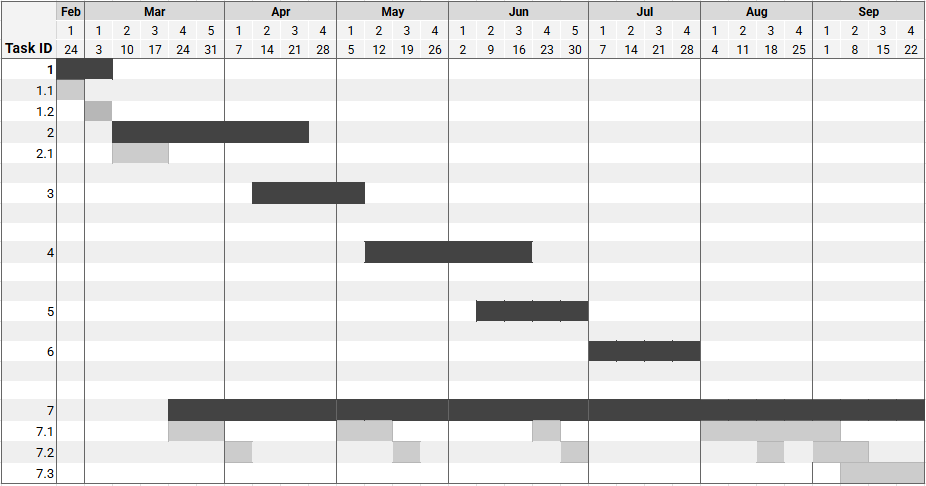
\includegraphics[width=\textwidth]{Chapters/Figures/Gantt.png}
    \caption{Gantt chart of the workplan}
    \label{fig:gantt}
\end{figure}

\section{Tasks \& Milestones}

\begin{table}[h!]
    \centering
    \footnotesize
    \begin{tabular}{|c|p{9cm}|c|}
    \hline
    \rowcolor[HTML]{C3C3C3} 
    \textbf{Task ID} & \textbf{Description} & \textbf{Dependency} \\ \hline
    \rowcolor[HTML]{E3E3E3} 
    \textbf{1}       & \textbf{Revision \& Consilidation of Elaboration Guidelines} & \textbf{}         \\ \hline
    \rowcolor[HTML]{FFFFFF} 
    1.1     & System Model \& Evaluation   & -         \\ \hline
    \rowcolor[HTML]{FFFFFF} 
    1.2     & Initial Specification of Components   & 1.1         \\ \hline
    
    %%%%%% PHASE 1 DEV %%%%%%
    \rowcolor[HTML]{E3E3E3} 
    \textbf{2}      & \textbf{Phase 1 Development \& Prototyping} & \textbf{}         \\ \hline
    \rowcolor[HTML]{FFFFFF} 
    2.1             & Setup Development Environment    & -        \\ \hline
    \rowcolor[HTML]{FFFFFF} 
    2.2             & Development of the first prototype    &  2.1         \\ \hline
    
    %%%%%% PHASE 1 TEST %%%%%%
    \rowcolor[HTML]{E3E3E3} 
    \textbf{3}      & \textbf{Phase 1 Evaluation \& Validation} & \textbf{}         \\ \hline
    \rowcolor[HTML]{FFFFFF} 
    3.1     & Development of the first tests   & 2.1         \\ \hline
    \rowcolor[HTML]{FFFFFF} 
    3.2     & Testing the Phase 1 Prototype    & 3.1         \\ \hline
    
    %%%%%% PHASE 2 DEV %%%%%%
    \rowcolor[HTML]{E3E3E3} 
    \textbf{4}       & \textbf{Phase 2 Development \& Prototyping} & \textbf{}         \\ \hline
    \rowcolor[HTML]{FFFFFF} 
    4.1     & Extending the first prototype    & 3.2         \\ \hline
  
    %%%%%% FINAL PHASE TEST %%%%%%
    \rowcolor[HTML]{E3E3E3} 
    \textbf{5}       & \textbf{Final Validation \& Experimental Evaluation} & \textbf{}         \\ \hline
    \rowcolor[HTML]{FFFFFF}
    5.1     & Testing the Final Prototype    & 4.1         \\ \hline
    \rowcolor[HTML]{FFFFFF} 
    5.2     & Optimizations and Final validations    & 4.1         \\ \hline
    \rowcolor[HTML]{FFFFFF} 
    5.2     & Final Observations    & 5.2, 5.3         \\ \hline
    %%%%%% REPORT %%%%%%

    \rowcolor[HTML]{E3E3E3} 
    \textbf{6}       & \textbf{Dissertation Report}     & \textbf{}      \\ \hline
    \rowcolor[HTML]{FFFFFF} 
    6.1       & Report Writing     &  -     \\ \hline
    \rowcolor[HTML]{FFFFFF} 
    6.2       & Report Revision    & -      \\ 
    \hline\rowcolor[HTML]{FFFFFF} 
    6.3       & Preparation for Presentation     & -      \\ 
    \hline
    
    \end{tabular}
    \caption{Overview of tasks and their dependencies as presented in Figure~\ref{fig:gantt}}
    \label{tab:task_table}
\end{table}

